\documentclass[12pt]{article}
\usepackage{sbc-template}
\usepackage{graphicx}
\usepackage{amsmath}
\usepackage{subfigure}
\usepackage{times,amsmath,epsfig}
\usepackage{graphicx,url}
  \makeatletter
  \newif\if@restonecol
  \makeatother
  \let\algorithm\relax
  \let\endalgorithm\relax
\usepackage[lined,algonl,ruled]{algorithm2e}
\usepackage{multirow}
\usepackage[brazil]{babel}
\usepackage[utf8]{inputenc}
\usepackage[pdftex]{hyperref}

\sloppy

\title{Algoritmos e Estruturas de Dados 3 \\ Trabalho Prático 5 \\
\huge{Cache}}
\date{November 22, 1963}


\author{André Taiar Marinho Oliveira}


\address{Departamento de Ciência da Computação -- Universidade Federal de Minas Gerais (UFMG)
\email{taiar@dcc.ufmg.br}
\\
\\ Novembro de 2010
}

\begin{document}

\maketitle

\begin{resumo}
\label{resumo}
Este relatório descreve um controlador de hierarquia de memórias e um simulador orientado a eventos para a geração de requisições de dados que estão gravados nesta memória. Foi simulado a requisição de dados que se encontravam em uma camada mais baixa (com alta latência) e utilizado um sistema de hierarquia de camadas de memória acima desta com o efeito de uma Cache para o sistema. Nessas camadas foram implementadas quatro políticas diferentes de Cache e aplicadas arbitráriamente sobre formatos igualmente arbitrários desse sistema. Como resultados pudemos perceber aspectos sobre o ganho da eficiência de sistemas que utilizam Cache e como combinações de diferentes tamanhos de caches e diferentes políticas de manejo de memória podem funcionar ajudando ou atrapalhando o sistema que a utiliza.
\end{resumo}

\section{Introdução}
\label{introducao}
\textit{"O ideal seria ter uma capacidade de memória infinitamente grande a ponto de qualquer word específica ... estar imediatamente disponível. ... Somos ... forçados a reconhecer a possibilidade de construir uma hierarquia de memórias, cada uma com capacidade maior que a anterior, mas com acessibilidade menos rápida."} \footnote{A. W. Burks, H. H. Goldstine e J. von Neumann - \textit{Preliminary Discussion of the Logical Design of an Electronic Computing Instrument, 1946}}

Hierarquia de memória é, basicamente, uma estrutura organizada em múltiplos níveis de memórias. Tais níveis de são diferenciados usualmente por duas dimensões: o tamanho (ou a capacidade de armazenamento daquele nível) e sua velocidade de acesso (ou sua latência - velocidade com a qual a memória disponibiliza o dado assim que ele é requisitado).

Neste trabalho desenvolvemos um simulador para hierarquias arbitrárias de memória. Nele, podemos definir o número de níveis que queremos, a capacidade de cada nível (em uma unidade chamada MUNITS), a velocidade em que cada nível responde à uma requisição (em uma unidade chamada TUNITS) e qual a política de manejo de memória aquele nível utiliza para lidar com os dados quando sua capacidade máxima de armazenamento for atingida. Com uma hierarquia definida, começamos a simular que dados são requeridos por algum sistema que estaria rodando sobre tal plataforma fazendo com que estes dados trafeguem pelo sistema.

Inicialmente, todos os dados se encontram em um nível inicial \textbf{0}, que funciona com uma capacidade e velocidade definidas independentemente da hierarquia de memória arbitrária que será simulada. Os dados são rquisitados sempre na camada de ID mais alto definida na hierarquia. Dessa forma, dois cenários são possíveis:

\begin{itemize}
  \item \textbf{HIT} - o dado é encontrado no nível requisitado;
  \item \textbf{MISS} - o dado não é encontrado no nível requisitado.
\end{itemize}

O tempo de resposta em que o dado foi encontrado equivale à velocidade da camada em que o dado foi encontrado. Quando acontece um HIT em uma camada em que um dado foi requisitado, ele é retornado e o HIT da camada é contabilizado. Quando acontece um MISS, o contabilizamos na camada e fazemos a requisição ao mesmo dado em um nível abaixo. As requisições são propagadas níveis abaixo à medida em que os MISS's acontecem até que seja requisitada ao nível 0 quando com certeza acontecerá o HIT. Nesse caso ele não é contabilizado.

Ao final da simulação, fazemos a razão entre os HIT e MISS contabilizados por cada camada e calculamos assim o MISS RATIO 
e o HIT RATIO:
\begin{center}
\[MissRatio = \frac{nMissCamada}{(nHitCamada + nMissCamada)}\]
\[HitRatio = \frac{nHitCamada}{(nHitCamada + nMissCamada)}\]
\end{center}

Contabilizamos também o tempo médio gasto em cada chamada à um dado no programa somando todos os tempos de resposta das camadas em acontece HIT e dividindo esse resultado pelo total de chamadas feitas ao programa.

\section{Solução Proposta}
\label{solucao_proposta}

Um algoritmo importante na solução é o que cria a estrutura de dados da hierarquia de memória que será simulado. Como ele depende da hierarquia setada na entrada, faremos a sua análise. Foi criado um tipo de dados para representar cada camada. A hierarquia de memória é representada por um vetor dessas camadas. Os dados que cada camada armazena são:

\begin{algorithm}[h!]
\begin{footnotesize}
$politica\longleftarrow$ guarda a política de manejo de memória utilizada pela camada\;
$capacidade\longleftarrow$ capacidade da camada\;
$velocidade\longleftarrow$ velocidade com que a camada responde\;
$ocupacao\longleftarrow$ o quanto da camada de memória já está sendo utilizada\;
$memoria[capacidade]\longleftarrow$ um vetor do tamanho da capacidade da memória para guardar os dados\;
\caption{Camada da Hierarquia}
\end{footnotesize}
\end{algorithm}

Para indicar que uma posição de memória está vazia, todas as células do vetor $memoria$ são inicialmente marcadas com o valor $-1$. Dessa forma, a complexidade do algoritmo para alocar essa estrutura é $O(n * m)$ onde $n$ é o número de camadas da cache e $m$ é o tamanho da maior capacidade de um nível de memória.

Com a estrutura de dados da hierarquia pronta, começamos a simulação requerendo o primeiro dado na primeira camada da hierarquia. A simulação começa como já descrito na sessão anterior e, em algum momento precisaremos gravar um dado em uma camada que já está cheia. Neste caso, devemos utilizar uma política de substituição de dados para escolher qual dado deve sair da memória para o mais novo entrar. Neste trabalho foram implementadas 4 políticas:

\begin{itemize}
  \item \textbf{LRU} - \textit{Least Recently Used}: o dado que foi utilizado à mais tempo é descartado;
  \item \textbf{LFU} - \textit{Least Frequently Used}: o dado que é utilizado menos frequentemente que os outros é descartado;
  \item \textbf{MRU} - \textit{Most Recently Used}: o dado que foi utilizado à menos tempo é descartado;
  \item \textbf{FIFO} - \textit{First In First Out}: os dados ficam em "fila" de modo que o que está a mais tempo na fila é descartado.
\end{itemize}

Para todas as políticas de substituição temos um algoritmo $O(n)$, porém a \textbf{FIFO} é mais custosa pois, para efeitos de simplificação do código, a fila é implementada como um arranjo fazendo com que todas as células do vetor tenham que ser copiadas para o seu próximo lugar na fila para a entrada de um novo dado.

Para as políticas \textbf{LRU} e \textbf{MRU}, é sempre armazenado o último tempo em que cada dado foi armazenado. Para a política \textbf{LFU} é armazenado o número de vezes em que cada dado foi acessado. Esses dados são armazenados na estrutura de simulação:

\begin{algorithm}[h!]
\begin{footnotesize}
$tempos[nObjetos] \longleftarrow$ armazena o último tempo em que cada objeto foi requisitado\;
$frequencias[nObjetos] \longleftarrow$ armazena quantas vezes um objeto foi requisitado\;
$hits[nCamadas] \longleftarrow$ armazena o número de hits de cada camada\;
$misses[nCamadas] \longleftarrow$ armazena o número de misses de cada camada\;
$reqTotal \longleftarrow$ armazena quantas chamadas à dados foram feitas na simulação\;
$tempoTotal \longleftarrow$ armazena o total de tempo gasto nas respostas às requisições\;
\caption{Estrutura de simulação}
\end{footnotesize}
\end{algorithm}

\section{Código}

\subsection{Módulos}
O programa foi separado em três módulos:
\begin{itemize}
\item \textbf{Camadas:} define a estrutura da hierarquia de memória utilizada na simulação descrevendo as operações e estruturas de cada camada de memória. Faz a alocação e desalocação de todas essas estruturas.
\item \textbf{Simulação:} implementa a parte de simulação do trabalho operando sobre a estrutura de hierarquia de memória. Faz a contagem dos dados da simulação como hits, misses e tempos de execução. Além disso contém a implementação de todas as políticas de cache do trabalho.
\item \textbf{Principal:} faz a leitura inicial do arquivo de entrada e trabalha com os módulos Camadas e Simulação. Faz a contagem do tempo de execução das partes principais do programa para análise de complexidade.
\end{itemize}

\subsection{Entrada e saída}
\subsubsection{Linha de comando}
O trabalho não necessita de argumentos para funcionar. Todos os dados serão passados pela entrada principal. Porém, para facilitar a execução e os testes do trabalho, um arquivo pode ser passado como fonte para a entrada padrão da seguinte forma:

\begin{verbatim}
#: ./tp5 < /caminho/para/o/arquivo
\end{verbatim}

\subsubsection{Formato da entrada}
Em um mesmo arquivo podem existir vários casos de teste. Em cada um deles, uma hierarquia diferente de memória pode ser definida bem como a série de chamados a objetos em memória. O formato de cada teste é:
\begin{verbatim}
nCamdas vCam1 cCam1 polCam1 ... vCamn cCamn polCamn cCam0
nTestes
Data1 Time1
Data2 Time2
...
Datat Timet
\end{verbatim}$nCamdas$ - número de camadas adicionais na hierarquia; \\
$vCam_{i}$ - velocidade da camada de id \textit{i}; \\
$cCam_{i}$ - capacidade de armazenamento da camada de id \textit{i}; \\
$polCam_{i}$ - política de cache utilizada pela camada de id \textit{i}; \\
$cCam_{0}$ - capacidade de armazenameno da camada 0; \\
$nTestes$ - número de chamadas a dados que será feito na simulação; \\
$Data_{i}$ - referência ao dado de id \textit{i}; \\
$Time_{i}$ - tempo em que o dado de id \textit{i} foi requisitado.

\subsubsection{Formato da saída}
A saída do programa é retornada na saída padrão do sistema informando a taxa de HIT e MISS de cada camada da hierarquia além do tempo médio total da simulação.
\begin{verbatim}
Camada 1 => Cache Hit Ratio = tHit1; Cache Miss Ratio = tMiss1
Camada 2 => Cache Hit Ratio = tHit2; Cache Miss Ratio = tMiss2
...
Camada n => Cache Hit Ratio = tHitN; Cache Miss Ratio = tMissN
------
Tempo de resposta médio por requisição = tMedResp T
\end{verbatim}$tHit_{i}$ - taxa de HIT da camada de id \textit{i}; \\
$tMiss_{i}$ - taxa de MISS da camada de id \textit{i}; \\
$tMedResp$ - tempo médio de resposta de todas as requisições.

\subsection{Compilação}
O compilador utilizado neste trabalho foi o GCC (adotado como padrão para a disciplina) e 
o comando para compilar o programa através do GCC é:
\begin{verbatim}
  #: gcc -o tp5 tp5.c camadas.c camadas.h simulacao.c simulacao.h
\end{verbatim}
caso estejam todos os arquivos dentro do mesmo diretório.

Como pedido na especificação, foi feito um arquivo Makefile com o qual é possível compilar
o programa com o comando: 
\begin{verbatim}
  #: make main
\end{verbatim}

E podemos compilar e executar o programa com o comando:
\begin{verbatim}
  #: make run
\end{verbatim}
que fará, além da compilação, com que o programa execute com uma entrada pequena.

\section{Avaliação Experimental}
\label{avaliacao_experimental}

\subsection{Qual o custo computacional da substituição de um objeto? Qual o custo em memória?}
\begin{tabular}{|c|c|c|}
\hline  & Custo Computacional & Custo em Memória \\ 
\hline lru & O(n) & O(n) \\ 
\hline lfu & O(n) & O(n) \\ 
\hline mru & O(n) & O(n) \\ 
\hline fifo & O(n) & O(n) \\ 
\hline 
\end{tabular} 
\subsection{Qual o custo total da execução da simulação? E o custo em memória?}
Já sei...
\subsection{Qual o custo computacional da substituição de um objeto? Qual o custo em memória?}
Plotar
\subsection{Qual o custo computacional da substituição de um objeto? Qual o custo em memória?}
Plotar
%\begin{figure}[ht!]
%\centering
%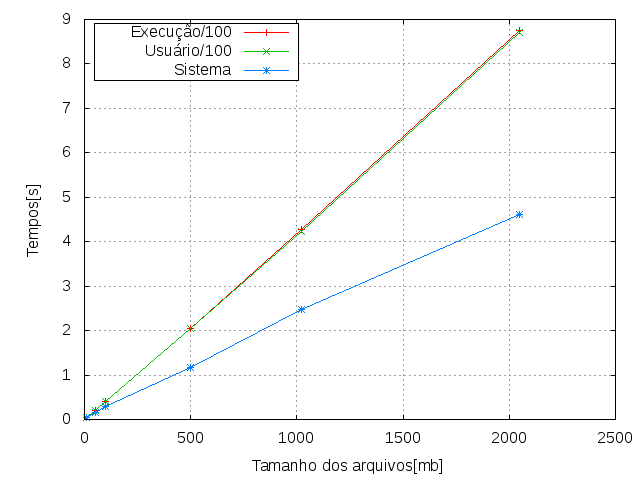
\includegraphics[width=3.5cm,height=2.8cm]{avaliacoes/testes.png}
%\label{img:resss}
%\caption{Gráfico dos tempos de execução}
%\end{figure}

\section{Conclusões}
\label{conclusao}

Por falta de tempo para implementar deixo aqui algumas idéias que fariam análises mais interessantes sobre o assunto e tornaria este trabalho mais proveitoso:
\begin{itemize}
  \item Uma boa idéia seria uti
\end{itemize}

\end{document}
